\section{Теоремы о стабилизации} \label{p21}
\paragraph{}
Рассмотрим математическую модель двухзвенного манипулятора. Манипулятор состоит из неподвижного основания и двух абсолютно жестких звеньев $G_1, G_2$. Элементы конструкции соединены между собой двумя идеальными цилиндрическими шарнирами $O_1,$ и $O_2$ таким образом, что оба звена могут совершать движения только в вертикальной плоскости. Центр масс $C_1$ звена $G_1$ лежит на луче $O_1 O_2.$ Положение центра масс $C_2$ звена $G_2$ не совпадает с положением шарнира $O_2$.

 \begin{figure}[h]
 	\centering
 	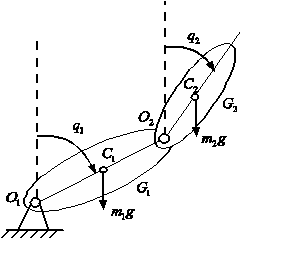
\includegraphics{manipulator}
 	\caption{Модель двузвенного манипулятора}
 	\label{fig:manip1}
 \end{figure}

Введем обозначения: $q_i (i=1, 2)$ --- углы поворотов звеньев манипулятора; $l_{q_i}$ --- длина отрезка $O_i C_i;$ $l_1$ --- длина отрезка $O_2 C_2;$ $m_i$  ---  масса   $i$-го звена;   $I_i$ --- момент инерции  $i$-го звена относительно оси шарнира $O_i;$ $g$ --- ускорение свободного падения.

Выражение для кинетечиской энергии манипулятора имеет в таком случае следующий вид:
\begin{equation}
T = \frac{1}{2} I_1 \dot q_1^2 + \frac12 m_2 l_1^2 \dot q_1^2 + \frac12 I_2 \dot q_2^2 + m_2 l_1 l_{q_2} \cos (q_2 - q_1) \dot q_1 \dot q_2.
\end{equation}

Составим уравнения Лагранжа второго рода:

\begin{equation}
\begin{cases}
\frac{d}{dt} (\frac{\partial T}{\partial \dot q_1}) - \frac{\partial T}{\partial q_1} = M_1 + U_1, 
\\
\frac{d}{dt} (\frac{\partial T}{\partial \dot q_2}) - \frac{\partial T}{\partial q_2} = M_2 + U_2,
\end{cases}
\end{equation}

где $M_i$ --- момент, создаваемый силой тяжести в $i$-м шарнире, $M_1 = (m_1 l_{g_1} + m_2 l_1) g \sin q_1, M_2 = m_2 l_{q_2} g \sin q_2, U_i $ --- управляющие воздействия.

Из выражения для кинетической энергии $T$ находим уравнения движения

\begin{equation}\label{2.1'}
\begin{cases}
(I_1 + m_2 l_1^2) \ddot q_1 + m_2 l_1 l_{g_2} \cos(q_2 - q_1) \ddot q_2 - m_2 l_1 l_{g_2} \sin(q_2 - q_1) \dot q_2^2 = \\ = (m_1 l_{g_1} + m_2 l_1) g \sin q_1 + U_1,
\\
I_2 \ddot q_2 + m_2 l_1 l_{g_2} \cos(q_2 - q_1) \ddot q_1 + m_2 l_1 l_{g_2} \sin(q_2 - q_1) \dot q_1^2 = m_2 l_{g_2} g \sin q_2 + U_2
\end{cases}
\end{equation}

Пусть $q=q(q_1, q_2)^{'}$ --– вектор обобщенных координат рассматриваемой механической системы и $X= {(q^0(t), \dot q^0(t)) : [t_0, + \infty) \to R^4, \|q^0(t)\| \le g_0, \|\dot q^0(t) \| \le g_1, \|\ddot q^0(t)\| \le g_2}$ есть заданное множество программных движений манипулятора в виде ограниченных дважды непрерывно дифференцируемых функций $q=q^0(t)$ с ограниченными производными при $t \in [t_0, + \infty).$ Символом $\| \cdot \|$   обозначена евклидова норма вектора.

Пусть $(q^0(t), \dot q^0(t)) \in X$ --- какое-либо программное движение, реализуемое программным управлением $U = U^0(t).$
Введем возмущения $x = q - q^0(t), \dot x = \dot q - \dot q^0(t)$

и составим уравнения возмущенного движения в векторно-матричном виде:

\begin{equation}
A^{(1)}(t, x) \ddot x = {\dot x^{'} C^{(1)}(t, x) \dot x} + Q^{(1)}(t,x) + Q^{(2)}(t, x, \dot x) + U^{(1)}, \label{2.2'}
\end{equation}

$$A^{(1)}(t, x) =
\begin{mpmatrix}
I_1 + m_2 l_1^2 && m_2 l_1 l_{g_2} \cos(q_2^0(t) - q_1^0(t) + x_2 - x_1) \\
m_2 l_1 l_{g_2} \cos(q_2^0(t) - q_1^0(t) + x_2 - x_1)  && I_2 \\
\end{mpmatrix}$$

$$ C^{(1)}(t,x)=(C_{(1)}^{(1)}(t,x), C_{(2)}^{(1)}), Q^{(1)}(t,x)=F(t,x)p(x), Q^{(2)}(t,x,\dot x)=D(t,x)\dot x, $$

$$ C_{(1)}^{(1)}(t, x) =
\begin{pmatrix}
0 && 0 \\
0 && m_2 l_1 l_{g_2} \sin(q_2^0(t) - q_1^0(t) + x_2 - x_1) \\
\end{pmatrix}, $$

$$C_{(1)}^{(2)}(t, x) =
\begin{pmatrix}
- m_2 l_1 l_{g_2} \sin(q_2^0(t) - q_1^0(t) + x_2 - x_1) && 0 \\
0 && 0\\
\end{pmatrix},$$

$$F(t, x) =
\begin{pmatrix}
f_{11}(t,x) && f_{12}(t,x) \\
f_{21}(t,x) && f_{22}(t,x)\\
\end{pmatrix},$$

$$p(x) =
\begin{pmatrix}
\sin(x_1/2) \\
\sin(x_2/2)\\
\end{pmatrix},$$

$$D(t, x) =
\begin{pmatrix}
0 && c_{22(1)}^{(1)}(t,x) \dot q_2^0(t) \\
c_{11(1)}^{(1)}(t,x) \dot q_1^0(t) && 0 \\
\end{pmatrix},$$

$f_{11}(t,x) = 2m_2l_1l_{g_2} \cos(x_2/2) (\ddot q_2^0(t) \sin(q_1^0(t) - q_2^0(t) + (x_1 - x_2)/2) - \\ - (\dot q_2^0(t))^2 \cos(q_1^0(t) - q_2^0(t) + (x_1 - x_2)/2)) + 2g(m_1 l_{g_2} + m_2 l_2) \cos(q_1^0(t) + x_1/2)$

$f_{12}(t,x) = - 2 m_2 l_1 l_{g_2} \cos(x_1/2) (\ddot q_2^0(t) \sin(q_1^0(t) - q_2^0(t) + (x_1 - x_2)/2) + \\ + (\dot q_2^0(t))^2 \cos(q_1^0(t) - q_2^0(t) + (x_1 - x_2)/2))$

$f_{21}(t,x) = 2 m_2 l_1 l_{g_2} \cos(x_2/2) (\ddot q_1^0(t) \sin(q_1^0(t) - q_2^0(t) + (x_1 - x_2)/2) + \\ + (\dot q_2^0(t))^2 \cos(q_1^0(t) - q_2^0(t) + (x_1 - x_2)/2))$

$f_{22}(t,x) = - 2m_2 l_1 l_{g_2} \cos(x_1/2) (\ddot q_1^0(t) \sin(q_1^0(t) - q_2^0(t) + (x_1 - x_2)/2) - \\ - (\dot q_2^0(t))^2 \cos(q_1^0(t) - q_2^0(t) + (x_1 - x_2)/2)) + 2 g m_2 l_{g_2} \cos(q_2^0(t) + x_2/2)$

$$ U^{(1)} = U - U^{0}(t) $$

Рассмотрим задачу построения управляющего воздействия  $ U^{(1)} = U^{(1)}(t, x, \dot x) $, $ U^{(1)} (t, 0, 0) \equiv 0 $, при котором бы невозмущенное движение $\dot x = x = 0$  системы (2.2) было бы равномерно асимптотически устойчиво, или, иными словами, управление $$U = U^0(t) + U^{(1)}(t, q-q^0(t), \dot q - \dot q^0(t))$$

обеспечивало бы стабилизацию программного движения $(q^0(t), \dot q^0(t)) \in X$  системы (2.1).

Рассмотрим решение задачи стабилизации в области 
$G = {(x, \dot x) \in R^4 : \|x\|<\epsilon, \|\dot x\|<\epsilon, \epsilon=const>0}$
с помощью непрерывного управления вида

$$U^{(1)}(x, \dot x) = B(\dot x + p(x))$$ \label{2.3'}     

где $B \in R^{2 \times 2}$ есть матрица коэффициентов усиления сигналов, подлежащая определению.
Возьмем для системы (2.2) вектор-функцию Ляпунова $V = (V^1, V^2)^{'}$  с коэффициентами вида $V^1 = \|p(x)\|, V^2 = \sqrt{(\dot x + p(x))^{'} A^{(1)}(t, x)(\dot x + p(x))}$.

Вычисляя производную по времени вектор-функции Ляпунова $V$ в силу системы (2.1), получим следующие оценки:
$$ \dot V^1 \le -mu_1 V^1 + \frac{m_1}{\lambda_1}, \dot V^2 le m_2 V^1 - \mu_2 V^2 + m_3 (V^1)^2 + m_4 (V^2)^2 + m_5 V^1 V^2, $$

где положительные постоянные $\mu_1, \mu_2, \lambda_1, m_i (i=1,2,...,5)$ определяются из следующих условий:

$$\lambda_1^2 = \frac{I_1 + m_2 l_1^2 + I_2 - \sqrt{(I_1 + m_2 l_1^2 - I_2)^2} + 4(m_2 l_1 l_{g_2})^2}{2}$$

$$\lambda_2^2 = \frac{I_1 + m_2 l_1^2 + I_2 + \sqrt{(I_1 + m_2 l_1^2 - I_2)^2} + 4(m_2 l_1 l_{g_2})^2}{2}$$

$\mu_1 =\frac12 \cos(\frac{\epsilon}{2}), m_1 = \frac12, m_2 = \max \frac{\lambda_2^2 + 2 \sqrt{\lambda_{max} [(D-F)^{'} (D-F)]}}{2 \lambda_1}, m_3 = \frac{m_2 l_1 l_{g_2}}{\lambda_1}, m_4 = \frac{2 m_2 l_1 l_{g_2}}{\lambda_1}, m_5 = \frac{3 m_2 l_1 l_{g_2}}{\lambda_1}, \mu_2 = \frac{-\lambda_2^2 - 4 g_1 m_2 l_q l_{g_2} - \lambda_{max} (B + B^{'})}{2 \lambda_2}$

Здесь $\lambda_max$ есть максимальное собственное значение соответствующей матрицы. 
Тогда для системы (2.1) можно построить следующую систему сравнения:

\begin{equation}\label{2.4'}
\dot u^1 = - \mu_1 u^1 + \frac{m_1}{\lambda_1} u^2, \dot u^2 = m_2 u^1 - \mu_2 u^2 + m_3 (u^1)^2 + m_4(u^2)^2 + m_5 u^1 u^2
\end{equation}

Согласно теореме сравнения об асимптотической устойчивости [5] из свойства асимптотической устойчивости нулевого решения системы сравнения (2.4) следует свойство равномерной асимптотической устойчивости нулевого решения системы (2.2). Получим условие асимптотической устойчивости нулевого решения системы (2.4) с областью притяжения $ {(u^1, u^2) \in R^2 : 0 \le u^1 \le \delta_1 = const>0, 0 \le u^2 \le \delta_2 = const>0} $ . Пусть найдется такое число $\gamma>0$, что выполняются соотношения:

\begin{equation}\label{2.5'}
\gamma = \frac{\delta_2 m_1}{\delta_1 \lambda_1 \mu_1}, \mu_2 > \frac{m_1}{\gamma \lambda_1 \mu_1} (m_2 + \delta_1 m_3) + m_4 \delta_2 + m_5 \delta_1
\end{equation}

Тогда можно показать, что функция $\widetilde{u}(t) = \max{(u^1(t), \delta_1 u^2(t)/ \delta_2)}$ будет монотонно стремиться к нулю при $t \to \infty$, и, значит, нулевое решение системы сравнения (2.4) будет асимптотически устойчиво.
При невозможности практической реализации программного управления стабилизацию программного движения можно осуществить при помощи разрывного управления вида

\begin{equation} \label{2.6'}
U^{(1)}(x, \dot x) = B \ sign(\dot x + p(x))
\end{equation}

Численное моделирование движения манипулятора при действии управлений (2.3) и (2.6) проводилось при следующих значениях параметров манипулятора и программной траектории:
$$ m_1 = 0,5 \text{кг}, m_2 = 0,3 \text{кг}, l_1 = 0,5 \text{м}, l_2 = 0,5 \text{м }, l_{g_1} = 0,25 \text{ м},  l_{g_2} = 0,3 м, I_1 = 0,01 \text{ кг} \cdot \text{м\textsuperscript{2}}, \\ I_2 = 0,006 \text{ кг} \cdot \text{м\textsuperscript{2}}, q_1^0(t) = \sin(0,5t), q_1^0(t) = \cos(0,5t) + \pi/2$$
На рисунках 2 и 3 представлены результаты моделирования при управлениях (2.3) и (2.6) соответственно. 

 \begin{figure}[h]
 	\centering
 	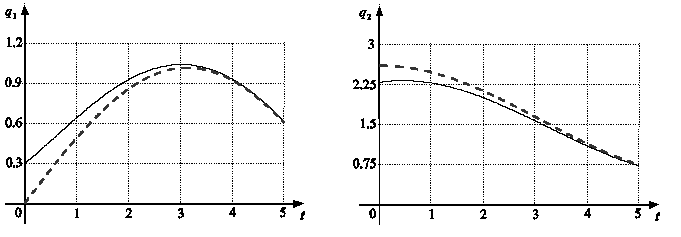
\includegraphics{model1}
 	\caption{Результаты моделирования при управлении (2.3)}
 	\label{fig:manip2}
 \end{figure}

 \begin{figure}[h]
 	\centering
 	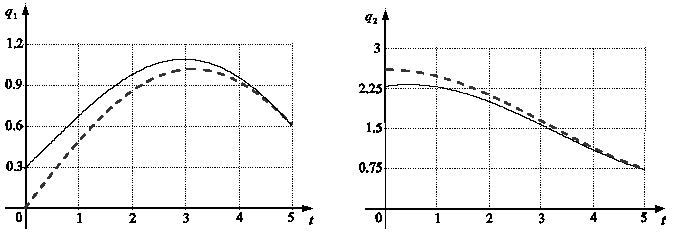
\includegraphics{model2}
 	\caption{Результаты моделирования при управлении (2.6)}
 	\label{fig:manip3}
 \end{figure}


